\chapter{Implementierung}
\label{chapter5}

Wie bereits erwähnt erfolgte die Implementierung in Java.
Damit für die Nutzung keine weiteren Installationen nötig sind,
wurden nur die Standardbibliotheken zur Umsetzung genutzt.
Der gesamte Source Code kann unter \href{https://github.com/lzfs/tsprocessor}{github/lzfs/tsprocessor}
abgerufen werden.
In diesem Kapitel wird vertiefend auf die Struktur des Tools eingegangen
und wichtige Aspekte der Implementierung betrachtet.


\section{Aufbau}
\label{5-Aufbau}
Der detailierte Aufbau des Tools kann dem Klassendiagramm in \autoref{fig:Classes} entnommen werden.
Hier wurde aus Gründen der Übersichtlichkeit auf Konstruktoren,
sowie Getter- und Setter-Methoden verzichtet.
\begin{figure}[p]
    \begin{center}
        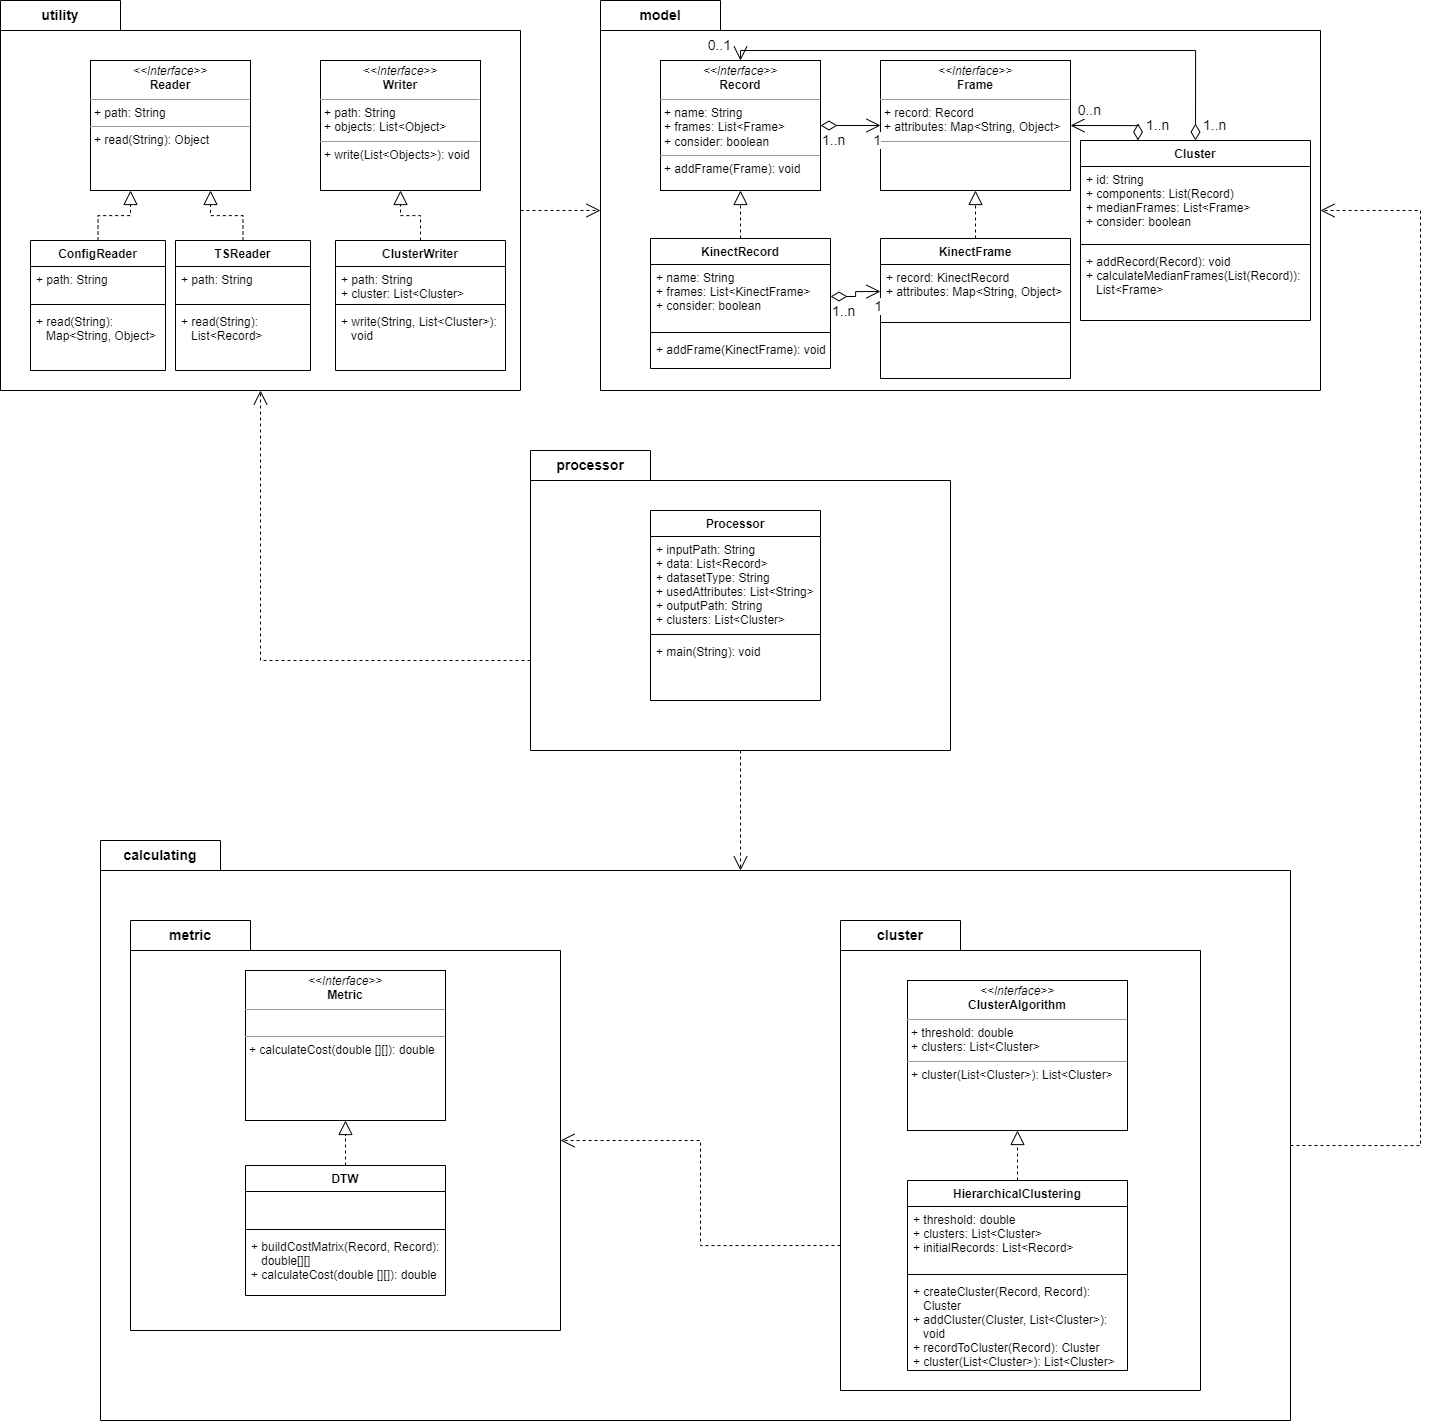
\includegraphics[width=0.6\textwidth]{classes.png}
    \end{center}
    \caption{Klassendiagramm des Tools.}
    \label{fig:Classes}
\end{figure}
Die wichtigen Aspekte dieser Architektur werden im Folgenden beschrieben.
Dabei entspricht die grobe Struktur der aus \autoref{4-Teilsysteme}.
Zum Start der Anwendung ist ein Aufrud der main-Methode des Processors nötig.
Dieser initialisiert zunächst geeignete Reader.
Das Reader-Interface wird konkret von den Klassen ConfigReader und DataReader implementiert.
Der ConfigReader dient lediglich dazu die Werte der Config-Datei einzulesen.
Dabei wird ein Properties Objekt zurückgeliefert,
mit dem auf die jeweiligen Werte zugegriffen werden kann.
Der DataReader liest die Kinect-Daten ein.
Ihm wird zunächst übermittelt, welche Attribute vorhanden sind,
durch welches Zeichen sie voneinander abgetrennt sind
und ob Frames übersprungen werden sollen,
um die Performanz zu verbessern.
Mit diesen Informationen liest er die Daten geeignet ein und liefert eine RecordImpl-Liste zurück.
Jeder Record enthält dabei eine Liste von FrameImpl.
Diese Datentypen sind die Implementierungen der entsprechenden Interfaces Record und Frame.
Sie können für Kinect-Daten genutzt werden.
Ein Frame enthält jeweils eine Map mit den vorhandenen Attributen die mithilfe der getValue-Methode
abgerufen werden können.
Ein weiterer Datentyp sind die Cluster.
Sie bestehen aus beliebig vielen, aber mindestens einem Record.
Hier werden die Methoden mergeWithCluster und mergeWithRecord angeboten.
Mit ihnen wird jeweils eine neue Komponente in das Cluster integriert.
Nach dem Einlesen und Abspeichern der Daten startet der Processor das Clustering.
Dazu wird eine Instanz von HierarchicalClustering, einer Implementierung von ClusterAlgorithm, erstellt.
Das Objekt erhält vom Prozessor alle wichtigen Informationen,
wie die initialen Records, den Threshold und die Attribute.
Da jedes Cluster am Anfang aus einem einzigen Record besteht,
wird die recordToCluster-Methode angeboten.
Mit ihr kann jeder der initialen Records transformiert und in der clusterImpls-Liste abgelegt werden.
Die cluster-Methode kümmert sich um den eigentlichen Cluster-Vorgang.
Dabei nutzt sie eine Instanz der Dtw-Klasse zur Berechnung von Kosten.
Sie implementiert das Metric-Interface und bietet daher die nötigen Methoden,
um die Kosten zwischen zwei Records, beziehungsweise deren Frame-Listen zu berechnen.
Dies wird durch den in \autoref{3-DTW} beschriebenen \ac{DTW}-Algorithmus realisiert.
Um auch Cluster mit Records vergleichen zu können bietet die Klasse zudem entsprechende
calculateMedianFrames-Methoden, die aus mehreren Frame-Listen eine neue erzeugt,
indem die Werte mithilfe von \ac{DTW} kombiniert werden.
Das genaue Verhalten von HierarchicalClustering und Dtw wird in \autoref{5-Codebeschreibung} näher beschrieben.
Nach dem Ende der Berechnungen liegen die gefundenen Cluster in der clusterImpl-Liste vor.
Sie können mit einem ClusterWriter geeignet in einer Textdatei abgespeichert werden.
Zudem kann eine Visualiserung mithilfe von VisualizerImpl erfolgen.
Die Klasse nutzt dazu einfache Java-AWT-Komponenten.
Der Wahrheitswert \emph{flipVisualization} gibt dabei an,
ob die Werte in x-Richtung gespiegelt werden sollen.
Dies ist nötig, da bei der Kinect das Koordinatensystem aus Nutzersicht erstellt wird.
In der Visualiserung führt dies dazu, dass die aufgezeichneten Bewegungen spiegelverkehrt erscheinen.
Der String \emph{attributeForBodyIdentification} dient dazu,
die unterschiedlichen Personen im Record korrekt darzustellen.

\section{Codebeschreibung}
\label{5-Codebeschreibung}

\begin{lstlisting}[language=Java, caption=Berechnung der Kosten.]
    public double calculateCost(
        List<FrameImpl> frames1,
        List<FrameImpl> frames2) {
        // add the calculated cost of each attribute to it
        double cost = 0;
        // calculate the cost for all attributes
        for (String attribute : this.usedAttributes) {
            // build the cost matrix for this attribute
            double[][] dtwMatrix = buildCostMatrix(
                frames1,
                frames2,
                attribute);
            // calculate and add the cost of this attribute
            cost += calculatePathCost(dtwMatrix);
        }
        return cost / this.usedAttributes.size();
    }
\end{lstlisting}


\begin{lstlisting}[language=Java, caption=Kostenmatrix.]
    private double[][] buildCostMatrix(
        List<FrameImpl> frames1,
        List<FrameImpl> frames2,
        String attribute) {
        double[] s = new double[frames1.size()];
        double[] t = new double[frames2.size()];

        int counter = 0;
        for (FrameImpl frame : frames1) {
            s[counter] = Double.parseDouble(frame.getValue(attribute));
            counter += 1;
        }
        counter = 0;
        for (FrameImpl frame : frames2) {
            t[counter] = Double.parseDouble(frame.getValue(attribute));
            counter += 1;
        }

        int n = s.length;
        int m = t.length;
        // filled with zeros by default
        double[][] dtwMatrix = new double[n + 1][m + 1];

        for (int i = 0; i < dtwMatrix.length; i++) {
            for (int j = 0; j < dtwMatrix[0].length; j++) {
                // filled with infinity by definition of dtw
                dtwMatrix[i][j] = Double.POSITIVE_INFINITY;
            }
        }
        // filled with 0 by definition of dtw
        dtwMatrix[0][0] = 0;

        for (int i = 1; i < dtwMatrix.length; i++) {
            for (int j = 1; j < dtwMatrix[0].length; j++) {
                // this is the default distance function
                double cost = Math.abs(s[i - 1] - t[j - 1]);
                
                double minTmp = Math.min(
                    dtwMatrix[i - 1][j],
                    dtwMatrix[i][j - 1]);
                double lastMin = Math.min(
                    minTmp,
                     dtwMatrix[i - 1][j - 1]);
                dtwMatrix[i][j] = cost + lastMin;
            }
        }
        return dtwMatrix;
    }
\end{lstlisting}

\begin{lstlisting}[language=Java, caption=Warping Path berechnen.]
    public double calculatePathCost(double[][] dtwMatrix) {
        int n = dtwMatrix.length - 1;
        int m = dtwMatrix[n - 1].length - 1;
        int pathCounter = 1;
        double cost = dtwMatrix[n][m];
        while (n != 0 && m != 0) {
            // dynamic time warping algorithm
            double minTmp = Math.min(dtwMatrix[n - 1][m], dtwMatrix[n][m - 1]);
            double lastMin = Math.min(minTmp, dtwMatrix[n - 1][m - 1]);
            cost += lastMin;
            if (lastMin == dtwMatrix[n - 1][m - 1]) {
                n = n - 1;
                m = m - 1;
            }
            else if (lastMin == dtwMatrix[n - 1][m]) {
                n = n - 1;
            }
            else if (lastMin == dtwMatrix[n][m - 1]) {
                m = m - 1;
            }
            pathCounter += 1;
        }
        return cost / pathCounter;
    }
\end{lstlisting}

\begin{lstlisting}[language=Java, caption=Hierarchisches Clustering.]
    public List<ClusterImpl> cluster() {
        List<ClusterImpl> result = new ArrayList<>();
        // initialize each record as a cluster and add it to the clusters list
        for (RecordImpl record : this.initialRecords) {
            this.clusterImpls.add(this.recordToCluster(record));
        }
        double currentMinimumCost;
        double cost;
        int mergeCandidate1;
        int mergeCandidate2;

        do {
            // reset for next loop iteration
            currentMinimumCost = this.dtw.calculateCost(    
                this.clusterImpls.get(0).getMedianFrames(),
                this.clusterImpls.get(1).getMedianFrames());
            cost = this.dtw.calculateCost(  
                this.clusterImpls.get(0).getMedianFrames(),
                this.clusterImpls.get(1).getMedianFrames());
            mergeCandidate1 = 0;
            mergeCandidate2 = 1;
            for (ClusterImpl clusterImpl1 : this.clusterImpls) {
                for (ClusterImpl clusterImpl2 : this.clusterImpls) {
                    if (
                        clusterImpl1 != clusterImpl2
                        && clusterImpl1.isConsider()
                        && clusterImpl2.isConsider()) {
                        if (this.calculatedCost.containsKey(
                            new ClusterKey(
                                clusterImpl1,
                                clusterImpl2))) {
                            cost = this.calculatedCost.get(
                                new ClusterKey(
                                    clusterImpl1,
                                    clusterImpl2));
                        }
                        else {
                            cost = this.dtw.calculateCost(
                                clusterImpl1.getMedianFrames(),
                                clusterImpl2.getMedianFrames());
                            this.calculatedCost.put(
                                new ClusterKey(
                                    clusterImpl1,
                                    clusterImpl2),
                                cost);
                        }
                        if (cost <= currentMinimumCost) {
                            /* if a cost smaller than the current minimum cost
                            is found this will be the new cost */
                            currentMinimumCost = cost;
                            mergeCandidate1 =
                                this.clusterImpls.indexOf(clusterImpl1);
                            mergeCandidate2 =
                                this.clusterImpls.indexOf(clusterImpl2);
                        }
                    }
                }
            }
            // if the minimum cost is still below the threshold we can continue
            if (
                currentMinimumCost < threshold
                && currentMinimumCost > this.minConst) {
                /* Combining mergeCandidate1 and mergeCandidate2
                has the lowest found cost.
                These two should therefore be merged together.
                Merge cluster2 into cluster1 and update the cluster list.
                Consider of cluster2 is set to false. */
                this.clusterImpls.get(mergeCandidate1).mergeWithCluster(
                    this.clusterImpls.get(mergeCandidate2));

                // create a copy of the map to avoid an exception
                Map<ClusterKey, Double> calculatedCostCopy = new HashMap<>();
                calculatedCostCopy.putAll(calculatedCost);

                /* remove all calculated costs from the map that contain
                cluster1 because it changed and therefore all cost values
                with this cluster have to be calculated again */
                for (Map.Entry<ClusterKey, Double> entry : calculatedCostCopy.entrySet()) {
                    /* ignore mergeCandidate2 because the consider
                    value of cluster2 is set to false */
                    if (entry.getKey().getCluster1().getId() == mergeCandidate1) {
                        for (ClusterImpl clusterImpl : clusterImpls) {
                            calculatedCost.remove(
                                new ClusterKey(
                                    this.clusterImpls.get(mergeCandidate1),
                                    clusterImpl));
                        }
                    }
                }
            }
        } while (
            currentMinimumCost < threshold
            && currentMinimumCost > this.minConst);
        /* clean up the list of found clusters by removing all clusters
        that shouldn't be considered anymore */
        for (ClusterImpl clusterImpl : this.clusterImpls) {
            if (clusterImpl.isConsider()) {
                result.add(clusterImpl);
            }
        }
        return result;
    }
\end{lstlisting}

\section{Abweichungen zur Konzeption}
\label{5-AbweichungenKonzeption}
An die Performanz der Anwendung wurden zwar keine besonderen Anforderungen gestellt
(\autoref{4-NichtFunktionaleAnforderungen}),
es zeigte sich aber schnell, dass bereits Datensätze mit mehreren Hundert Records zu langen Bearbeitungszeiten führen.
Daher wurden zwei Funktionen integriert die sich diesem Problem annehmen sollen.
Zum einen werden die berechneten Kosten in einer Map abgespeichert,
um wiederholte Berechnungen in darauffolgenden Schritten zu vermeiden.
Als Key der jeweiligen Map-Einträge dient ein Objekt der Klasse ClusterKey.
Sie implementiert das Comparable-Interface und sorgt dafür,
dass zwei Cluster zusammen als Key einer Map verwendet werden können.
Dies spart viele Berechnungsschritte,
da beinahe alle Werte im Vergleich zum vorherigen Iterationsschritt gleich bleiben.
Lediglich jene Kosten an denen die neu zusammengeführten Cluster beteiligt waren,
sowie die Kosten mit dem neuen Cluster müssen neu berechnet werden.
Zum anderen gibt es die Möglichkeit jeden zweiten Frame der Records zu ignorieren.
Dies geschieht, indem der Parameter \emph{skipFrames} in der config-Datei auf \emph{true} gesetzt wird.
Damit ist in der Regel weiterhin ein sinnvolles Clustering möglich,
wobei die Anzahl der Berechnungsschritte drastisch reduziert werden kann.
Hier ist zu erwähnen, dass aber definitiv Informationen verloren gehen.
Diese Option sollte daher nur bei sehr großen Datenmengen genutzt werden.

Zudem wurde abweichend zur Konzeption ein primitiver \emph{Visualizer} ergänzt,
da sonst die Analyse der Cluster mühsam über Kinect Studio erfolgen muss.
Er stellt die Laufwege der gefundenen Cluster aus der Vogelperspektive dar.
Für jedes Cluster wird ein Verzeichnis erstellt.
Darin werden die einzelnen Komponenten visualisiert.